\documentclass[a4paper,10pt,fleqn]{article}

\usepackage{layout}

\newboolean{STANDALONE}
\setboolean{STANDALONE}{false}

\newboolean{EMBED}
\setboolean{EMBED}{false}


\setboolean{EMBED}{true}

\title{Dokumentation BLDC}
\newcommand{\BrushlessPath}{src}
\newcommand{\DasAndereTeam}{T27 }
\newcommand{\BLDCTeams}{T27 und T32}
\newcommand{\BLDCcollab}{Dieses Kapitel ist eine Zusammenarbeit der Gruppen \BLDCTeams. }

\begin{document}

\maketitle
\clearpage
\tableofcontents
\clearpage

\ifSTANDALONE
\section{Hardware}
\fi
\ifEMBED
\subsection{Hardware}
\fi
Die Elektrotechnik-Studierenden aus mehreren Gruppen haben sich
zusammengeschlossen um gemeinsame Probleme anzugehen. Dabei handelt es sich
um die Ansteuerung, die benötigte Hard- und Software um Motoren anzusteuern
und gegebenenfalls zu regeln. In diesem Zusammenschluss wurde drei Gruppen
gebildet, um Lösungen für DC-, Stepper- und Brushless-Motoren auszuarbeiten.
Die Idee besteht darin, dass nicht jede Gruppe für dasselbe Problem wo
möglich denselben Lösungsansatz verfolgt, sondern die Ressourcen kombiniert,
Synergien nutzt um eine bessere Lösung zu erarbeiten. Auf diese Weise kann
das Team übergreifende Arbeiten im Rahmen der \enquote{PREN} erlernt und
geübt werden. Somit wird Idee der Interdisziplinarität im erweiterten Sinn
Rechnung getragen. Die Gruppen und deren Mitglieder sind in der Tabelle 
\ref{tab:pren-et-overview} aufgeführt.
\begin{table}[h!]
	\centering
	\begin{tabular}{l l}
		Projekt		& Team \\
		\hline
		DC Motoren	& 39 \\
		Schrittmotor	& 27, 38 \\
		BLDC Motor	& 27, 32 \\
	\end{tabular}
	\caption{Übersicht der PREN-ET Projektgruppen}
	\label{tab:pren-et-overview}
\end{table}

\newpage
\subsection{Brushless Motoransteuerung}
    % Dieses Kapitel ist eine Zusammenarbeit der Gruppen \BLDCTeams. 
    \BLDCcollab
    \subsubsection{Theorie der Ansteuerung}
        \begin{wrapfigure}{r}{0.50\textwidth}
           	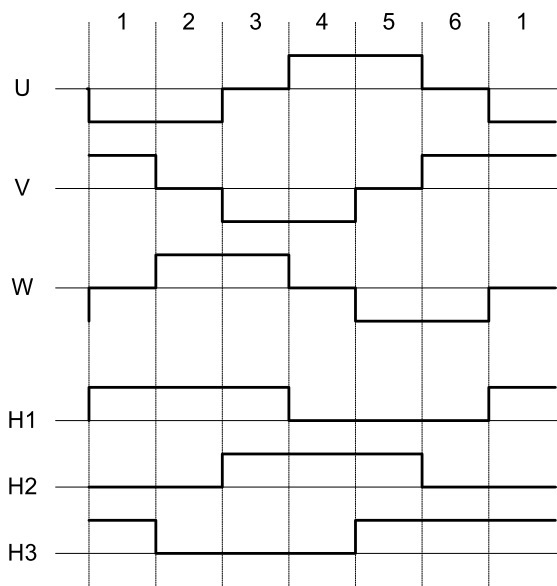
\includegraphics[scale=0.45]{\BrushlessPath/Bilder/ZeitlicheHallSensorAnsteuerung.jpg}
           	\caption[Zeitliche Darstellung der Ansteuerung mit 
                Hall-Sensoren]{Zeitliche Darstellung der Ansteuerung mit 
                Hall-Sensoren \cite{AppNote:BrushlessuC}}
           	\centering
            \label{abb:ZeitlicheAnsteuerungBrushlessMotor}
        \end{wrapfigure}
        Brushless-Motoren sind Synchron-Drehstrom-Motoren. Das heisst, sie 
        werden mittels eines kontinuierlichen Drehfeldes in Bewegung gesetzt. 
        Dabei ist darauf zu achten, dass der Läufer dem Drehfeld synchron 
        folgen kann, daher der Name. Falls der Läufer dem Drehfeld aus irgend 
        einem Grund nicht folgen kann, so wird keine Spannung vom Rotor in die 
        Statorwicklungen induziert, die der Erregerspannung entgegenwirkt. 
        Daraus folgt, dass ein immenser Strom fliesst, der nur von der 
        Wicklungsimpedanz des Motors begrenzt wird.\\
        \\
        Es gibt hauptsächlich drei Methoden das Drehfeld zu generieren und zu 
        regeln. Die eine und einfache Methode ist die Zwangskommutierung. 
        Dabei wird ein Drehfeld erzeugt und dem Motor aufgezwungen. Der Läufer 
        muss dem Drehfeld folgen können. Dabei ist ein maximaler Winkel 
        zwischen dem Feld und dem Läufer von 90$^\circ$ zulässig. Wird deser 
        Winkel überschritten, wird der Motor zum Stillstand kommen mit den 
        erwähnten Folgen.\\
        \\
        Die zweite Methode zur Regelung ist mittels drei Hallsensoren, die im 
        Motor integriert sind. Dies macht den Motor aufwändiger und 
        dementsprechend teurer. Die Regelung mit Hallsensoren ist 
        verhältnismässig einfach, da je nach den Signalen die einzelnen Spulen 
        direkt angesteuert werden können. Der Zusammenhang zwischen der 
        Ansteuerung und den Hall-Sensorsignalen ist in Abbildung 
        \ref{abb:ZeitlicheAnsteuerungBrushlessMotor} ersichtlich. Dabei stehen 
        $U$, $V$ und $W$ für die Phasenströme und $H_1$, $H_2$ und $H_3$ für die 
        entsprechenden Signale der Hallsensoren. Dieser Darstellung ist zu 
        entnehmen, dass jedesmal, wenn ein Hallsensor eine Änderung anzeigt, 
        ein Nulldurchgang im entsprechenden Stromverlauf stattgefunden hat. 
        Dies ist der Zeitpunkt, zu dem die Kommutierung durchgeführt werden 
        muss.\\
        \\
        Die dritte Möglichkeit ist, indem man einen virtuellen Sternpunkt 
        bildet und mittels Komparatoren die Sternpunktdurchgänge detektiert. 
        In der Controller-Logik muss der Zeitunterschied der Kommutierung 
        bis zum durchschreiten des Sternpunktes gemessen werden. Diese Zeit 
        muss nochmal abgewartet werden bevor die Kommutierung durchgeführt 
        werden.
    
    \subsubsection{Neuer Ansatz}
        \begin{wrapfigure}{r}{0.40\textwidth}
           	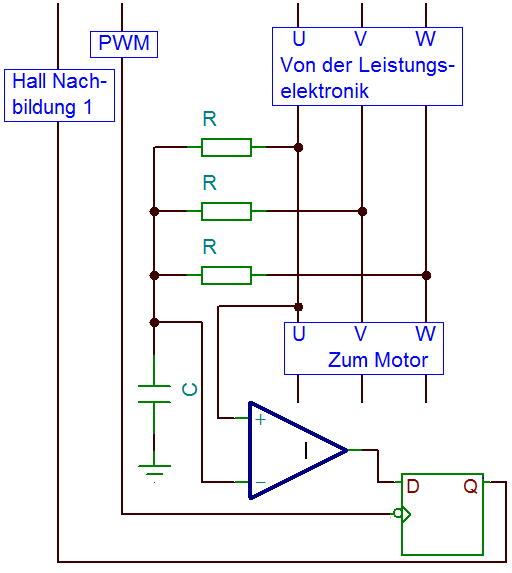
\includegraphics[scale=0.46]{\BrushlessPath/Bilder/PrinzipDerRekonstruktion.png}
           	\centering
           	\caption[Schema des Rekonstruktionsprinzip]{Schema des Rekonstruktionsprinzip \cite{HSLU:Pluess}}
            \label{abb:PrinzipRekonstruktion}
        \end{wrapfigure}
        In einem modifizierten Ansatz wird versucht, ob die Hall-Sensorsignale 
        aus den Ansteuerungen des Motors gewonnen werden können. Hierzu wird 
        eine Schaltung pro Phase benötigt, um die Nulldurchgänge beim 
        virtuellen Sternpunkt detektieren zu können. Die Abbildung 
        \ref{abb:PrinzipRekonstruktion} zeigt die Schaltung, mit der dies 
        realisiert werden kann. Mit dem Flip-Flop kann die PWM aus dem 
        Sensorsignal unterdrückt werden. Diese rekonstruierten 
        Hall-Sensor-Signale können direkt logischen verknüpft und genutzt 
        werden, um den Motor mittels einer Dreiphasen-H-Brücke anzusteuern 
        \cite{HSLU:Pluess}. Anhand des zeitlichen Verlaufs, der aus Abbildung 
        \ref{abb:ZeitlicheAnsteuerungBrushlessMotor} zu entnehmen ist, und der 
        Ansteuerung einer H-Brücke ergibt sich die Wahrheitstabelle, die in 
        Abbildung \ref{abb:WahrheitstabelleAnsteuerung} abgebildet ist. Das 
        Signal $U_h$ symbolisiert den Highside-Transistor der Phase U auf der 
        H-Brücke und die $U_l$ entspricht dem Lowside-Transistor.\\      
        
        \begin{figure}[h!]
            \begin{tabular}{ccc||cc|cc|cc||c}
                 $H_1$ & $H_2$ & $H_3$ & $U_h$ & $U_l$ & $V_h$ & $V_l$ & $W_h$ & $W_l$ & Illegal\\
            \hline 0   &   0   &   0   &   0   &   0   &   0   &   0   &   0   &   0   &   1\\
                   0   &   0   &   1   &   0   &   0   &   0   &   1   &   1   &   0   &   0\\
                   0   &   1   &   0   &   0   &   1   &   1   &   0   &   0   &   0   &   0\\
                   0   &   1   &   1   &   0   &   1   &   0   &   0   &   1   &   0   &   0\\
                   1   &   0   &   0   &   1   &   0   &   0   &   0   &   0   &   1   &   0\\
                   1   &   0   &   1   &   1   &   0   &   0   &   1   &   0   &   0   &   0\\
                   1   &   1   &   0   &   0   &   0   &   1   &   0   &   0   &   1   &   0\\
                   1   &   1   &   1   &   0   &   0   &   0   &   0   &   0   &   0   &   1\\
            \end{tabular}
           	\centering
           	\caption{Wahrheitstabelle der Ansteuerung} 
            \label{abb:WahrheitstabelleAnsteuerung}
        \end{figure}
        \parindent 0pt Die Tabelle in Abbildung 
        \ref{abb:WahrheitstabelleAnsteuerung} kann pro Signal zu folgenden 
        logischen Verknüpfung vereinfacht werden\\
        \\
        \begin{tabular}{ccc}
            $U_h = H_1 \wedge \bar{H_2}$ & $V_h = H_2 \wedge \bar{H_3}$ & $W_h = \bar{H_1} \wedge H_3$\\
            $U_l = \bar{H_1} \wedge H_2$ & $V_l = \bar{H_2} \wedge H_3$ & $W_l = H_1 \wedge \bar{H_3}$
        \end{tabular}

\newpage
  \subsubsection{Aufbaubeschreibung}
        \begin{wrapfigure}{r}{0.55\textwidth}
           	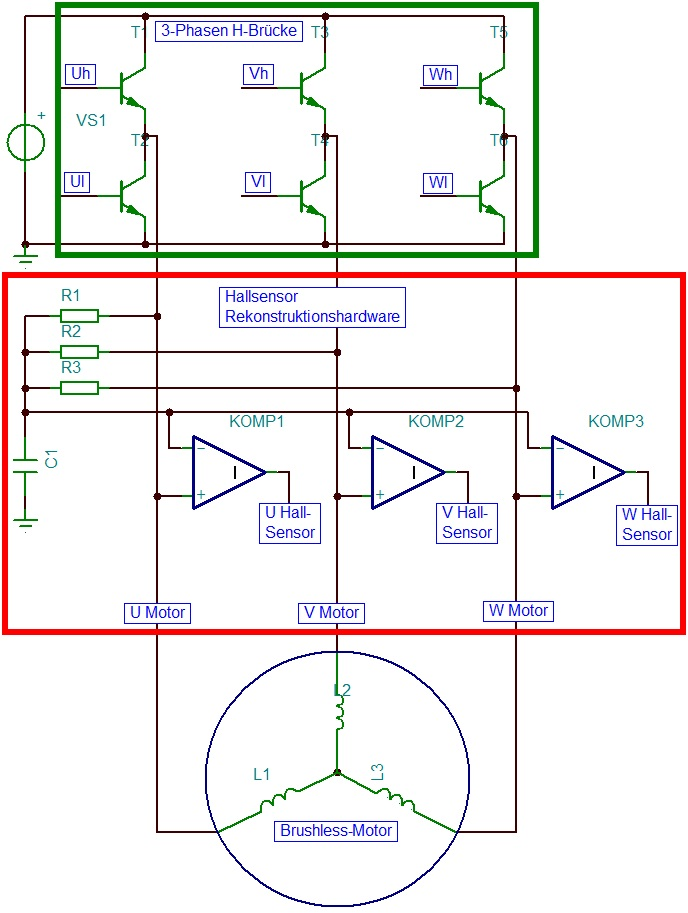
\includegraphics[scale=0.4]{\BrushlessPath/Bilder/MotoransteuerungSchema.jpg}
           	\centering
           	\caption{Schema des Brushless-Versuchsaufbaus}
            \label{abb:MotoransteuerungSchema}
        \end{wrapfigure}
        Das Schema des gesamten Aufbaus des Tests ist in der Abbildung 
        \ref{abb:MotoransteuerungSchema} abgebildet. Die 3-Phasen H-Brücke 
        oben im grünen Rechteck wird direkt vom FPGA angesteuert. Die Hardware 
        dieser Brücke ermöglicht eine voll galvanisch getrennte Ansteuerung 
        mit 3.3V Logikpegeln. Diese Brücke wurde zur Verfügung gestellt und 
        verwendet. Die Rekonstruktion der Hallsensoren-Signale findet im rot 
        markierten Teil des Aufbaus statt. Dieser Part wurde auf einer 
        Laborplatte aufgebaut und zusammen gelötet. Die so generierten Signale 
        $U_{Hallsensor}$, $V_{Hallsensor}$, $W_{Hallsensor}$ werden einem FPGA 
        geliefert. Anhand dieser Signale steuert das FPGA die 
        H-Brücken-Transistoren mittels der Signale $U_h$, $U_l$, $V_h$, $V_l$, 
        $W_h$, $W_l$. Die im FPGA enthaltene Konfiguration sind simple 
        AND-Verknüpfungen, die die anliegenden Signale sehr schnell und 
        effizient verarbeiten. Auf diese Weise ist es möglich, den Motor sehr 
        schnell anzusteuern.\\
        \\
        In der Abbildung \ref{abb:MessplatzAufbau} ist der gesamte Aufbau 
        abgebildet. Man beachte die markierten Felder. Am unteren linken Rand 
        ist der Motor befestigt. In der Mitte des Bildes ist die Hardware, mit 
        welcher die Hallsensoren Signale rekonstruiert werden. Die generierten 
        Signale werden dem FPGA in der unteren linken Ecke zugeführt. Diese 
        Signale werden logisch verknüpft und danach werden die sechs Signale 
        generiert um die H-Brücke in der oberen rechten Hälfte anzusteuern. 
        Diese wiederum treiben den Motor an.
        \begin{figure}[h!]
        %\vspace{-16pt}
           	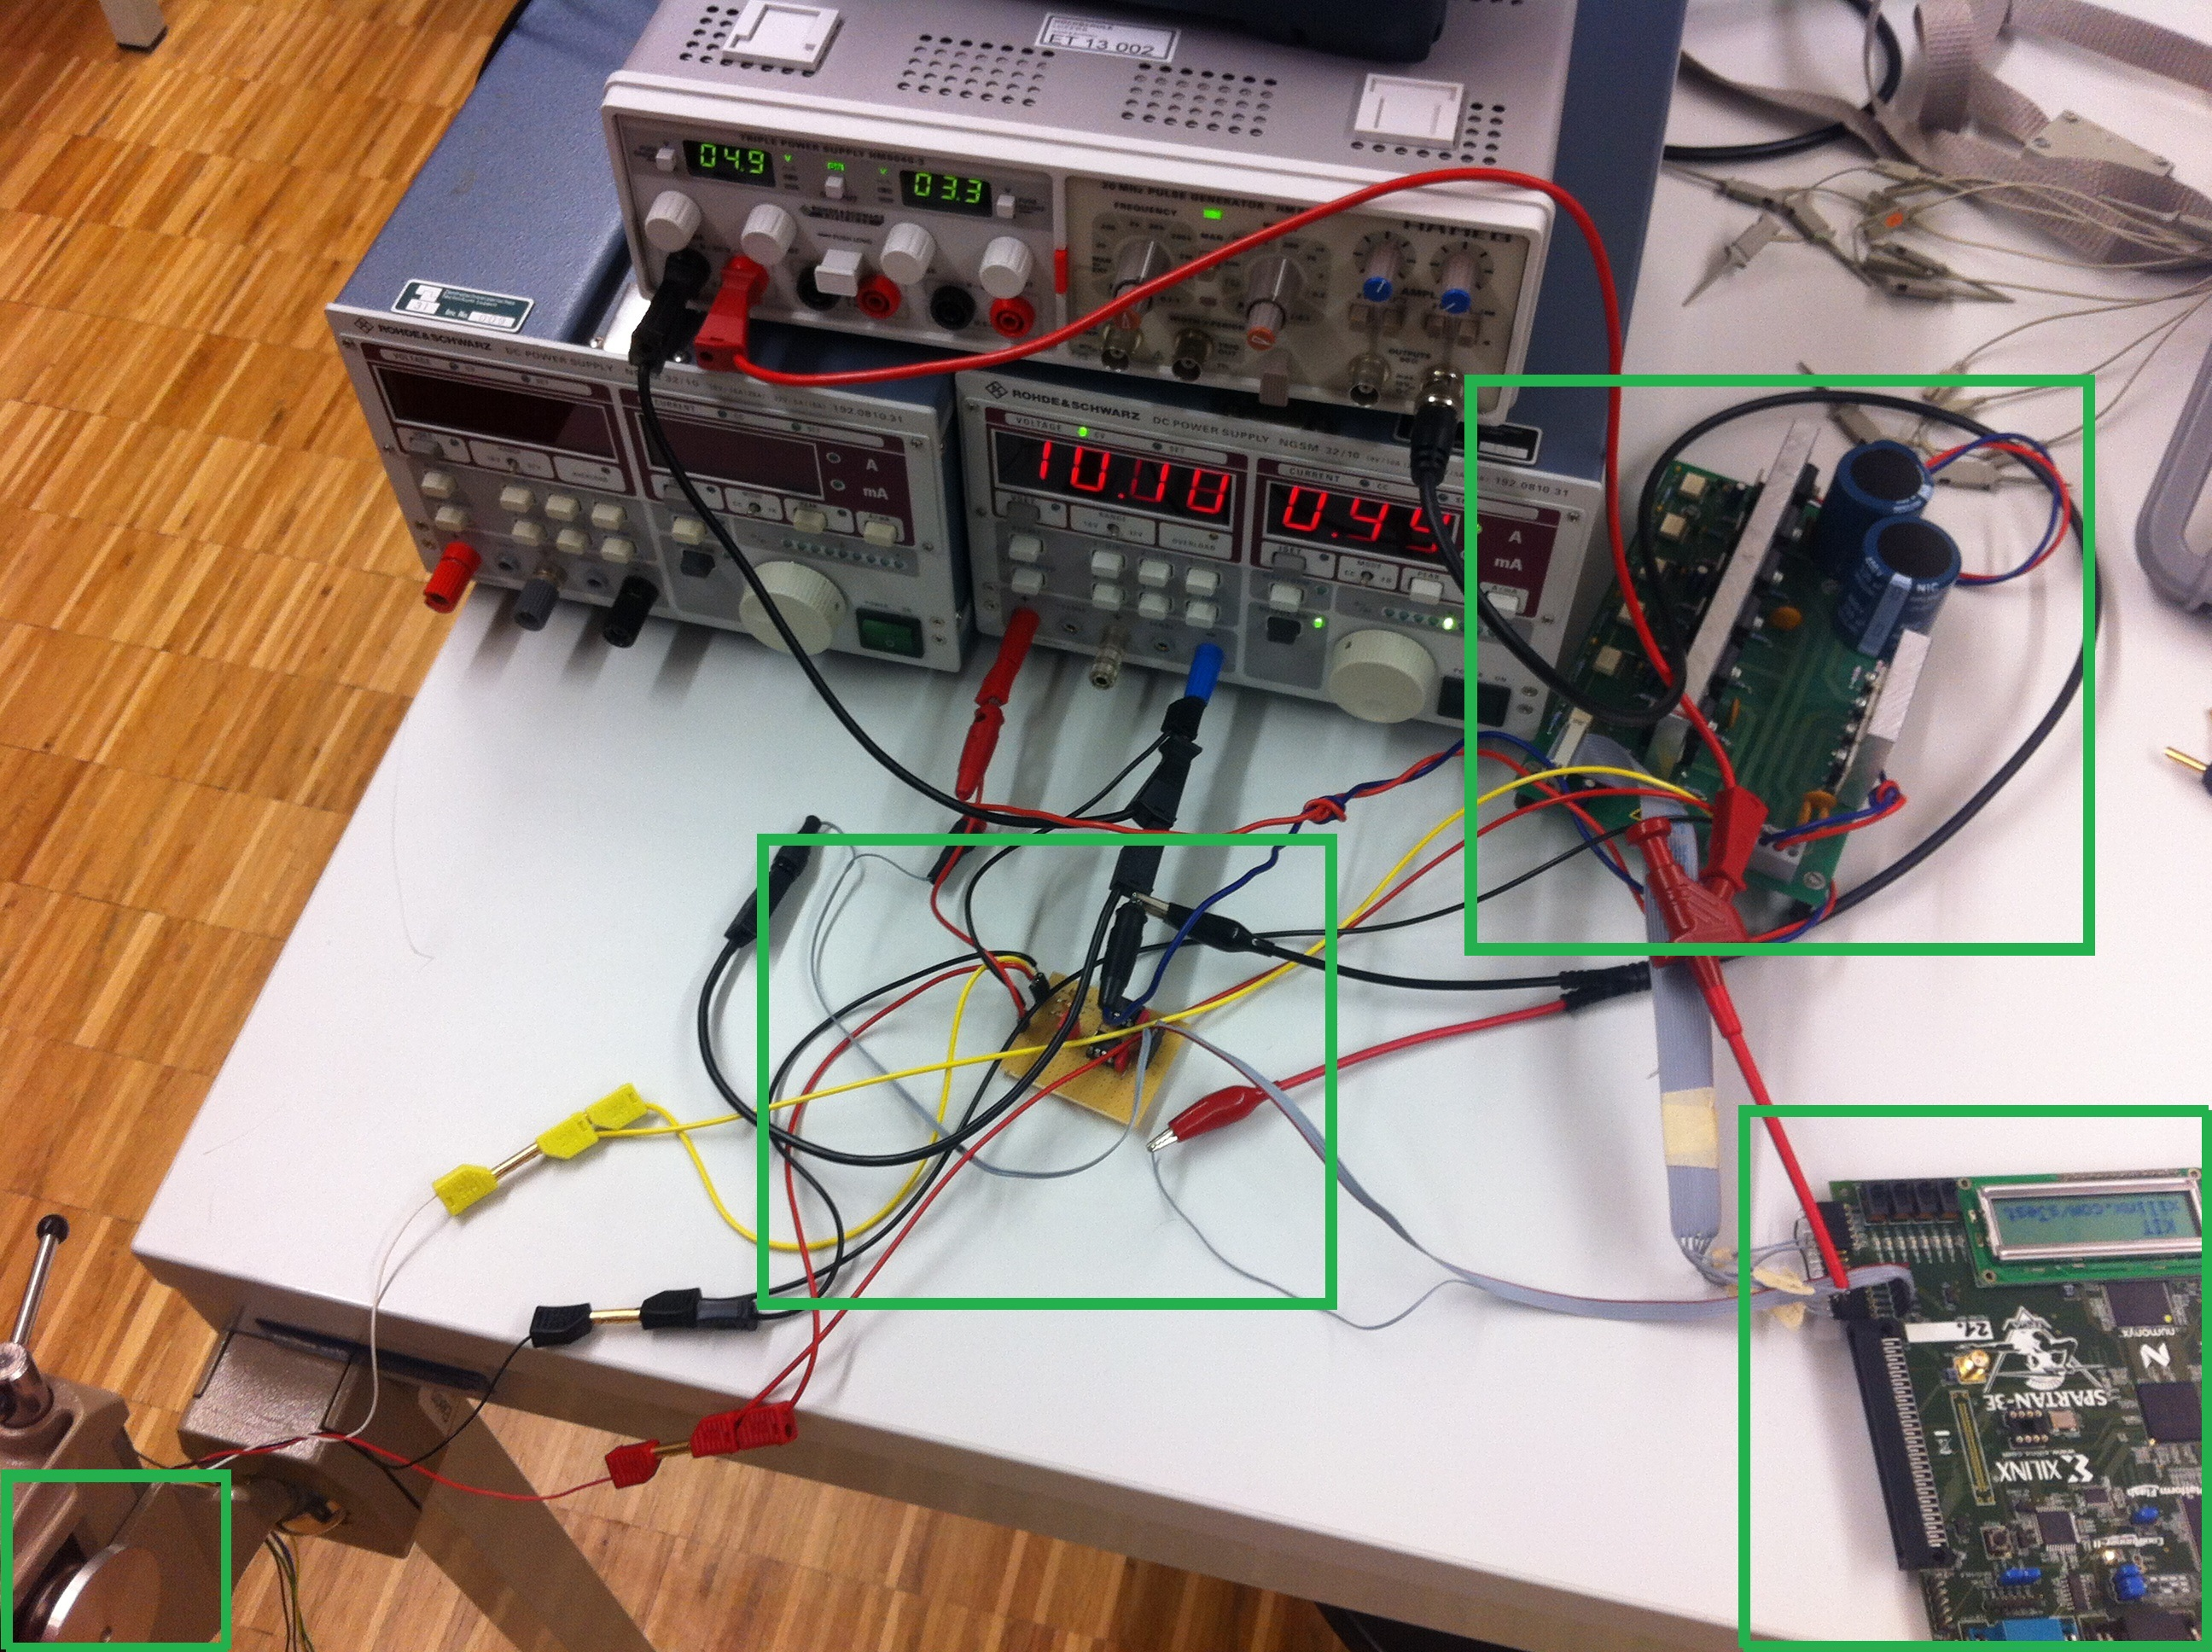
\includegraphics[scale=0.14]{\BrushlessPath/Bilder/MessplatzAufbau.jpg}
           	\centering
           	\caption{Testaufbau} 
            \label{abb:MessplatzAufbau}
        %\vspace{-10pt}
        \end{figure}\\
        Die im FPGA enthaltene Logik basiert auf der Wahrheitstabelle, die in 
        Abbildung \ref{abb:WahrheitstabelleAnsteuerung} abgebildet ist.
        
    \subsubsection{Messmittel}
        \begin{zebratabular}{lll}
            \rowcolor{gray} Gerät &
                Typ &
                Nummer \\
            Speisegerät & 
                Rohde \& Schwarz NGSM 32/10 &
                Inv. Nr. 009 \\
            Oszilloskop &
                Agilent MSO6052A &
                Inz. Nr. 44 S/N: MY44001903 \\
            Mainframe &
                Hameg HM8001-2 &
                SN: 059520046 \\
            Speisegerät &
                Hameg HM8040-3 &
                SN: 015405014 \\
            Pulsgenerator &
                Hameg HM8035 &
                Inv. Nr. 44 \\
        \end{zebratabular}


\newpage

\begin{flushleft}
    \renewcommand{\refname}{Literatur- und Quellenverzeichnis}
%        \{\refname}{Quellenverzeichnis}
    \bibliography{src/BLDC_Source}{} %!!! Kein Leerzeichen nach dem , !!!!
\end{flushleft}

\end{document}
